\section{Results}
\label{sec:results}

\subsection{Predictive benchmarking and the cost of leakage}
\cref{tab:bench} reports contemporaneous ozone estimation across the three evaluation
protocols and the baseline ladder. The result is unambiguous: apparent skill is an
artifact of the protocol. The gradient-boosted model attains $R^2=0.412$ under the
i.i.d.\ random split, but this collapses to $R^2=0.251$ under the blocked temporal Q4
holdout and $R^2=0.304$ under spatial leave-stations-out, falling further to
$R^2=0.219$ under the strict temporal$\times$spatial intersection
(\cref{fig:leakage}). The $\sim$$0.16$--$0.19$ absolute $R^2$ gap between the random
split and the blocked/grouped protocols is pure spatio-temporal leakage: neighbouring
hours of the same station, near-duplicates of one another, leak across the random
train/test boundary \citep{kaufman2012leakage,roberts2017cv}.

Two baselines frame the honest skill. The linear Ridge reference is weak everywhere
($R^2\le 0.17$), confirming that the signal the boosted model captures is genuinely
non-linear; but a trivial \emph{lag-1 persistence} predictor attains $R^2=0.794$ on the
same temporal holdout. The learned model is thus valuable only where persistence is
unavailable---namely spatial interpolation to unmonitored sites---and is \emph{beaten
by doing nothing} for temporal gap-filling. The diurnal-seasonal climatology
($R^2=0.041$) shows that static station behaviour alone explains almost none of the
hour-to-hour variance.

\begin{table}[t]
  \centering
  \caption{Leakage-safe predictive benchmarking of contemporaneous ozone estimation.
  All preprocessing fit on the training fold only; hyper-parameters fixed a priori.
  Persistence and the diurnal-seasonal mean are defined only for the temporal
  holdout. Lower RMSE/MAE and higher $R^2$ are better.}
  \label{tab:bench}
  \begin{tabular}{llrrr}
    \toprule
    Protocol & Model & $R^2$ & RMSE & MAE \\
    \midrule
    \multirow{2}{*}{Random split (leaky)}
      & XGBoost                       & 0.412 & 23.72 & 14.90 \\
      & Ridge ($L_2$)                 & 0.167 & 28.21 & 18.63 \\
    \midrule
    \multirow{4}{*}{Blocked temporal (Q1--Q3 $\to$ Q4)}
      & XGBoost                       & 0.251 & 26.49 & 16.19 \\
      & Ridge ($L_2$)                 & 0.082 & 29.32 & 18.78 \\
      & Diurnal-seasonal mean         & 0.041 & 29.98 & 20.04 \\
      & Persistence (lag-1)           & \textbf{0.794} & \textbf{13.88} & \textbf{5.57} \\
    \midrule
    \multirow{2}{*}{Spatial leave-stations-out (5-fold)}
      & XGBoost                       & 0.304 & 27.94 & 18.45 \\
      & Ridge ($L_2$)                 & 0.159 & 28.33 & 18.73 \\
    \midrule
    Temporal $\times$ spatial (strict)
      & XGBoost                       & 0.219 & 30.00 & 18.41 \\
    \bottomrule
  \end{tabular}
\end{table}

\begin{figure}[t]
  \centering
  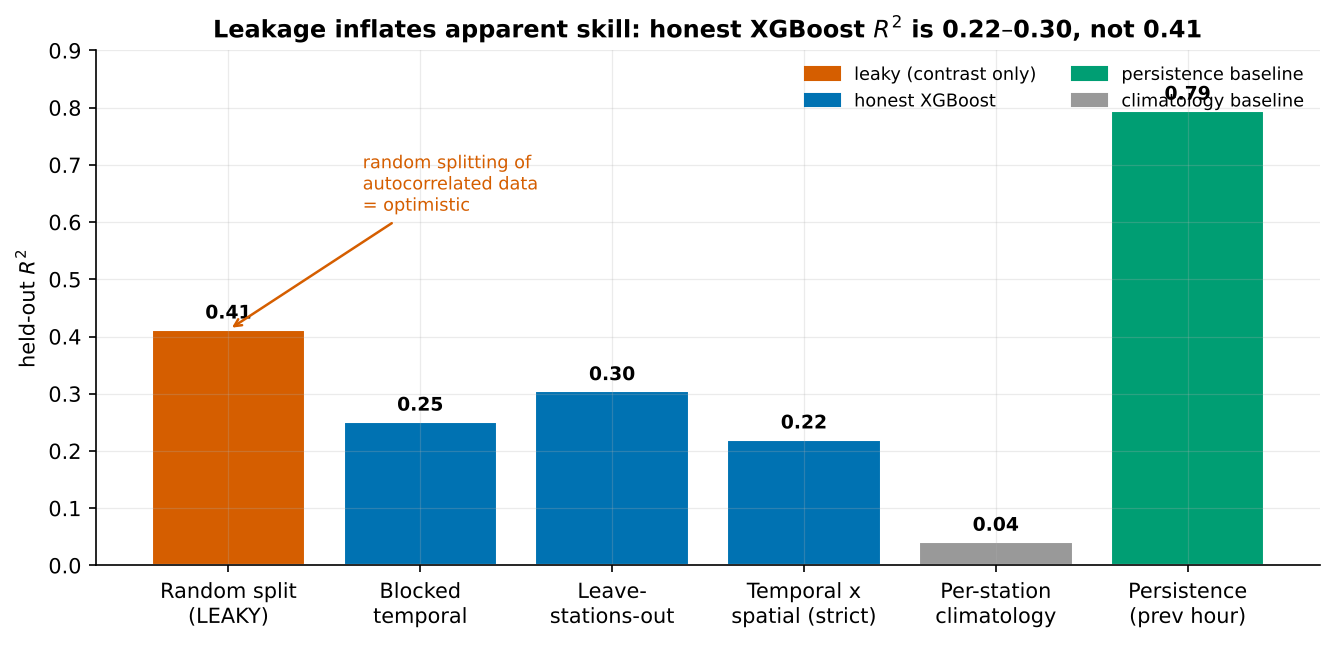
\includegraphics[width=0.95\linewidth]{fig2_leakage_benchmark.png}
  \caption{Held-out $R^2$ for contemporaneous ozone by evaluation protocol. Random
  splitting of autocorrelated telemetry inflates skill to $0.41$; honest blocked and
  grouped protocols give $0.22$--$0.30$. A previous-hour persistence baseline (green)
  dominates for temporal gap-filling.}
  \label{fig:leakage}
\end{figure}

\subsection{Meteorology ablation}
Stripping covariate groups under the blocked temporal protocol isolates their
contributions. A weather-only model attains $R^2=0.140$ and a pollutant-only model
$R^2=0.132$, while the full model reaches $R^2=0.251$. The incremental value of the six
pollutants \emph{beyond} meteorology is therefore only $\Delta R^2\approx+0.117$: most
of the explainable ozone variance is meteorological, and the chemical covariates add a
small, though non-trivial, increment. Any downstream ``mechanistic'' reading must
account for the fact that meteorology, not chemistry, carries the bulk of the signal.

\subsection{Recovered structure and its atmospheric interpretation}
The bootstrap-stabilized DirectLiNGAM structure is shown in \cref{fig:dag}. Of all
candidate edges, exactly one is both bootstrap-stable (selection frequency $1.0$) and
survives the inclusion of meteorology as exogenous nodes: the negative edge
$\mathrm{NO}\rightarrow\mathrm{O_3}$, with standardized coefficient
$-0.138\pm0.007$ in the pollutant-only model, attenuating to $-0.108$ once temperature,
humidity, wind and pressure are included. This is the chemical signature of
\emph{localized} titration, $\mathrm{NO}+\mathrm{O_3}\rightarrow\mathrm{NO_2}+\mathrm{O_2}$,
expected in fresh, NO-rich urban (traffic-dominated) air \citep{sillman1999,
monks2015ozone}: ambient NO destroys ozone locally. Crucially, this is \emph{not}
regional photochemical production, which is governed by VOC oxidation that these data
cannot observe. The remaining high-frequency edges
($\mathrm{NO}\rightarrow\mathrm{NO_2}$, $+0.40$; $\mathrm{NO_2}\rightarrow\mathrm{PM_{2.5}}$,
$+0.23$; and the CO combustion edges, frequency $0.91$) are consistent with shared
combustion co-emission but involve unit-indeterminate species (\cref{sec:units}) and,
for the particulate edges, collapse once meteorology is included---evidence that the
pollutant-only graph is confounded by the boundary layer (\cref{sec:gate}).
SO\textsubscript{2} edges are unstable (frequency $\le0.5$) and are not retained.

\begin{figure}[t]
  \centering
  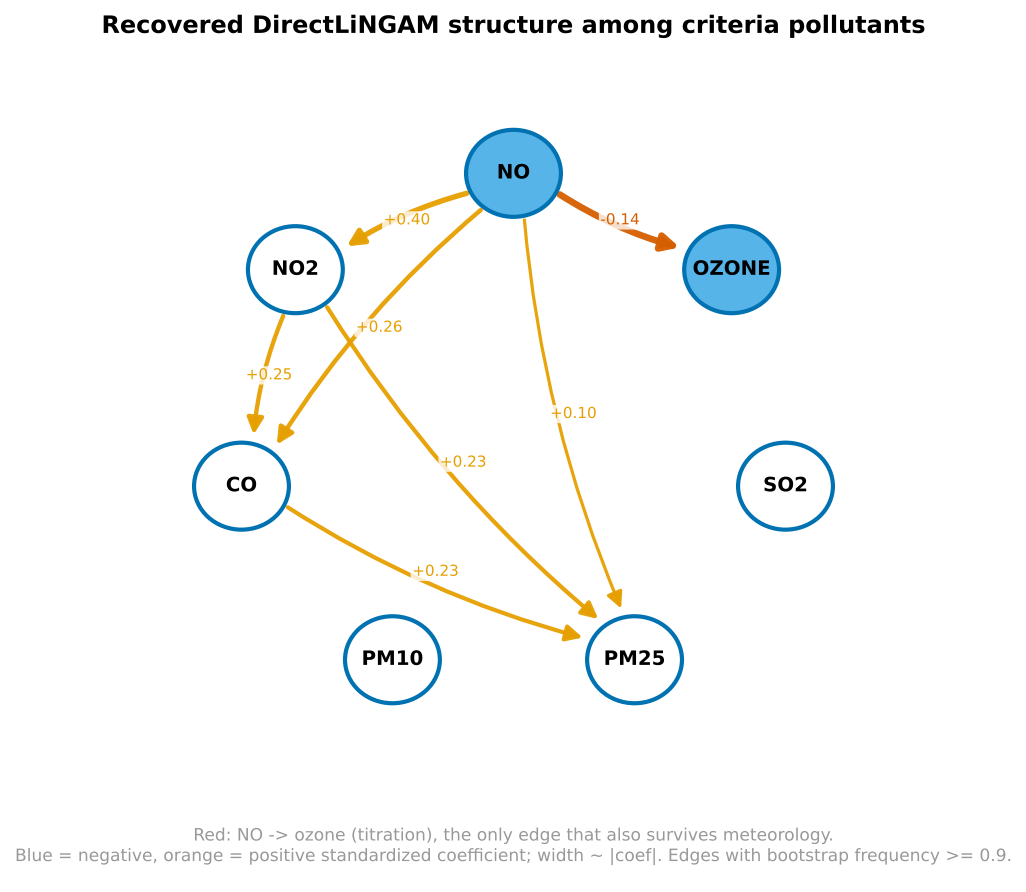
\includegraphics[width=0.78\linewidth]{fig3_causal_dag.png}
  \caption{Recovered DirectLiNGAM structure (bootstrap frequency $\ge 0.9$). Only
  $\mathrm{NO}\rightarrow\mathrm{O_3}$ (red, negative) is both stable and robust to
  meteorological confounding. Edge width scales with $|$coefficient$|$;
  SO\textsubscript{2} carries no stable edge.}
  \label{fig:dag}
\end{figure}

\subsection{Empirical Pareto frontier versus the NSGA-II archive}
\cref{lem:pareto} predicts that the true frontier is a one-dimensional segment with
$z_{\mathrm{NO_2}}=z_{\mathrm{CO}}=z_{\min}$. We computed this exact segment in closed
form and audited the $19$ saved NSGA-II candidate policies against it
(\cref{tab:pareto}, \cref{fig:pareto}). Every one of the $19$ heuristic policies is
dominated by the exact frontier---a $100\%$ dominance rate---with a mean objective-space
gap of $0.046$ (maximum $0.298$) in standardized PM\textsubscript{2.5}, a generational
distance of $\mathrm{GD}=0.084$ \eqref{eq:gd}, and a hypervolume error of
$\mathrm{HVE}=6.6\%$ \eqref{eq:hve}. The heuristic fails precisely as
\cref{cor:pareto} anticipates: unaware of the boundary structure, NSGA-II scatters
interior points rather than driving the reducible coordinates to their bound. For a
linear surrogate, the metaheuristic is not merely unnecessary---it is strictly inferior
to a closed-form solution that any analyst can write down.

\begin{table}[t]
  \centering
  \caption{Audit of the heuristic NSGA-II archive against the exact analytical Pareto
  frontier of the fitted linear surrogate (\cref{lem:pareto}). Objectives are
  standardized; gaps are Euclidean in objective space.}
  \label{tab:pareto}
  \begin{tabular}{lr}
    \toprule
    Quantity & Value \\
    \midrule
    Heuristic candidate policies audited          & $19$ \\
    Policies dominated by the exact frontier       & $19$ ($100\%$) \\
    Mean gap to frontier (std.\ PM\textsubscript{2.5}) & $0.046$ \\
    Maximum gap to frontier                        & $0.298$ \\
    Generational distance, $\mathrm{GD}$           & $0.084$ \\
    Hypervolume error, $\mathrm{HVE}$              & $6.6\%$ \\
    Exact frontier: $z_{\mathrm{NO_2}}^\star=z_{\mathrm{CO}}^\star$ & $z_{\min}=-2$ \\
    Exact frontier endpoints $(z_{\mathrm{O_3}},z_{\mathrm{PM_{2.5}}})$
      & $(0,-0.89)\to(0.25,-1.08)$ \\
    \bottomrule
  \end{tabular}
\end{table}

\begin{figure}[t]
  \centering
  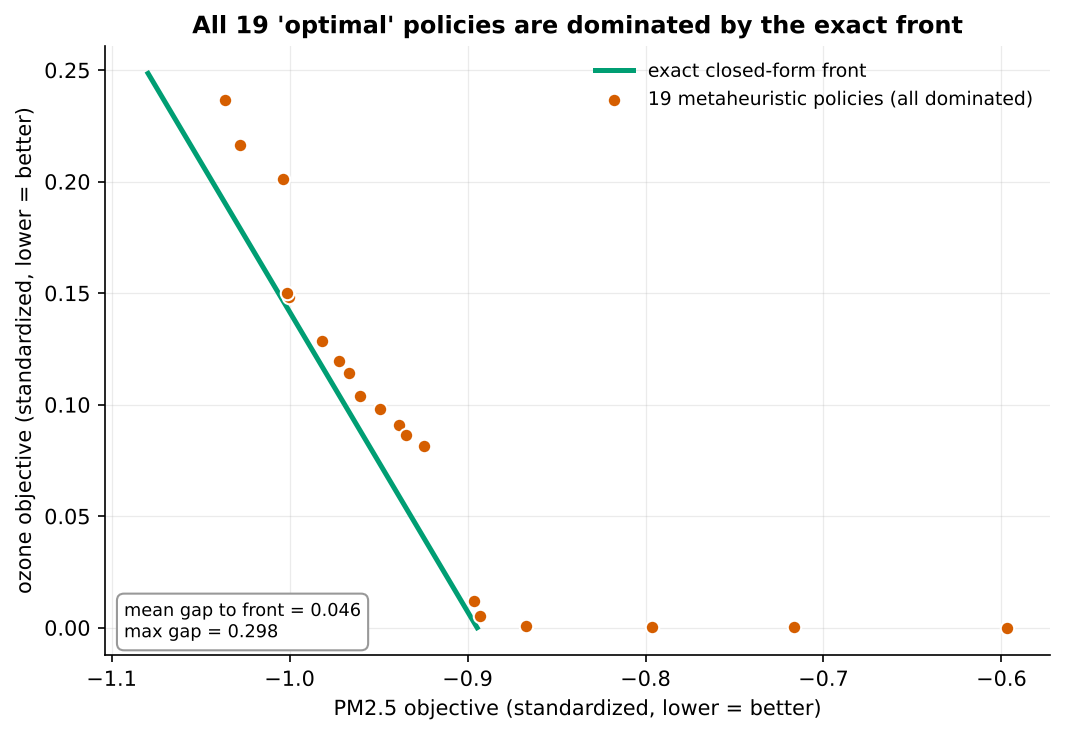
\includegraphics[width=0.72\linewidth]{fig4_analytic_pareto.png}
  \caption{The $19$ NSGA-II ``optimal'' policies (orange) against the exact closed-form
  Pareto frontier (green) of the linear surrogate. All heuristic points are dominated.}
  \label{fig:pareto}
\end{figure}

\subsection{Model explainability}
\cref{fig:shap} shows the global SHAP importance ranking \citep{lundberg2017shap,
lundberg2020treeshap} for the ozone model. Relative humidity and temperature dominate,
followed by NO as the leading chemical covariate---mirroring both the meteorology
ablation and the single stable structural edge. We stress the epistemic status of this
agreement: SHAP and DirectLiNGAM are two summaries of the \emph{same} fitted model and
data. Their concordance on the sign and prominence of NO is \emph{internal
consistency}, not independent validation; it cannot license a causal claim that the
leakage-safe and confounding analyses do not already support.

\begin{figure}[t]
  \centering
  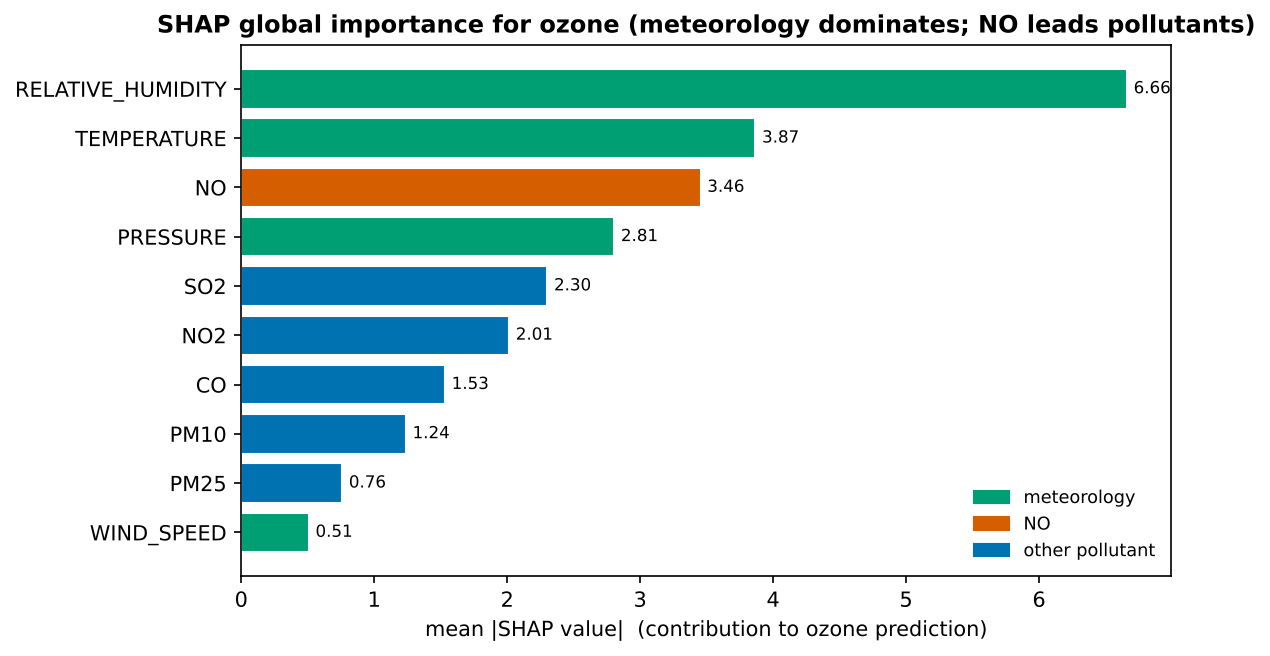
\includegraphics[width=0.9\linewidth]{fig5_shap_importance.png}
  \caption{Global SHAP importance (mean $|$SHAP$|$) for ozone estimation. Meteorology
  dominates; NO is the leading chemical covariate, consistent with
  \cref{fig:dag}. Per-sample attributions were not retained, so a beeswarm is not shown.}
  \label{fig:shap}
\end{figure}
